\batchmode
\documentclass[twoside]{book}

% Packages required by doxygen
\usepackage{fixltx2e}
\usepackage{calc}
\usepackage{doxygen}
\usepackage[export]{adjustbox} % also loads graphicx
\usepackage{graphicx}
\usepackage[utf8]{inputenc}
\usepackage{makeidx}
\usepackage{multicol}
\usepackage{multirow}
\PassOptionsToPackage{warn}{textcomp}
\usepackage{textcomp}
\usepackage[nointegrals]{wasysym}
\usepackage[table]{xcolor}

% Font selection
\usepackage[T1]{fontenc}
\usepackage[scaled=.90]{helvet}
\usepackage{courier}
\usepackage{amssymb}
\usepackage{sectsty}
\renewcommand{\familydefault}{\sfdefault}
\allsectionsfont{%
  \fontseries{bc}\selectfont%
  \color{darkgray}%
}
\renewcommand{\DoxyLabelFont}{%
  \fontseries{bc}\selectfont%
  \color{darkgray}%
}
\newcommand{\+}{\discretionary{\mbox{\scriptsize$\hookleftarrow$}}{}{}}

% Page & text layout
\usepackage{geometry}
\geometry{%
  a4paper,%
  top=2.5cm,%
  bottom=2.5cm,%
  left=2.5cm,%
  right=2.5cm%
}
\tolerance=750
\hfuzz=15pt
\hbadness=750
\setlength{\emergencystretch}{15pt}
\setlength{\parindent}{0cm}
\setlength{\parskip}{3ex plus 2ex minus 2ex}
\makeatletter
\renewcommand{\paragraph}{%
  \@startsection{paragraph}{4}{0ex}{-1.0ex}{1.0ex}{%
    \normalfont\normalsize\bfseries\SS@parafont%
  }%
}
\renewcommand{\subparagraph}{%
  \@startsection{subparagraph}{5}{0ex}{-1.0ex}{1.0ex}{%
    \normalfont\normalsize\bfseries\SS@subparafont%
  }%
}
\makeatother

% Headers & footers
\usepackage{fancyhdr}
\pagestyle{fancyplain}
\fancyhead[LE]{\fancyplain{}{\bfseries\thepage}}
\fancyhead[CE]{\fancyplain{}{}}
\fancyhead[RE]{\fancyplain{}{\bfseries\leftmark}}
\fancyhead[LO]{\fancyplain{}{\bfseries\rightmark}}
\fancyhead[CO]{\fancyplain{}{}}
\fancyhead[RO]{\fancyplain{}{\bfseries\thepage}}
\fancyfoot[LE]{\fancyplain{}{}}
\fancyfoot[CE]{\fancyplain{}{}}
\fancyfoot[RE]{\fancyplain{}{\bfseries\scriptsize Generated by Doxygen }}
\fancyfoot[LO]{\fancyplain{}{\bfseries\scriptsize Generated by Doxygen }}
\fancyfoot[CO]{\fancyplain{}{}}
\fancyfoot[RO]{\fancyplain{}{}}
\renewcommand{\footrulewidth}{0.4pt}
\renewcommand{\chaptermark}[1]{%
  \markboth{#1}{}%
}
\renewcommand{\sectionmark}[1]{%
  \markright{\thesection\ #1}%
}

% Indices & bibliography
\usepackage{natbib}
\usepackage[titles]{tocloft}
\setcounter{tocdepth}{3}
\setcounter{secnumdepth}{5}
\makeindex

% Hyperlinks (required, but should be loaded last)
\usepackage{ifpdf}
\ifpdf
  \usepackage[pdftex,pagebackref=true]{hyperref}
\else
  \usepackage[ps2pdf,pagebackref=true]{hyperref}
\fi
\hypersetup{%
  colorlinks=true,%
  linkcolor=blue,%
  citecolor=blue,%
  unicode%
}

% Custom commands
\newcommand{\clearemptydoublepage}{%
  \newpage{\pagestyle{empty}\cleardoublepage}%
}

\usepackage{caption}
\captionsetup{labelsep=space,justification=centering,font={bf},singlelinecheck=off,skip=4pt,position=top}

%===== C O N T E N T S =====

\begin{document}

% Titlepage & ToC
\hypersetup{pageanchor=false,
             bookmarksnumbered=true,
             pdfencoding=unicode
            }
\pagenumbering{alph}
\pagenumbering{arabic}
\hypersetup{pageanchor=true}

%--- Begin generated contents ---
\chapter{Demo problem\+: Deformation of a string under tension, using Kirchhoff-\/\+Love Beam elements.}
\label{index}\hypertarget{index}{}\hypertarget{index_q}{}\section{A few quick questions...}\label{index_q}
Since {\ttfamily oomph-\/lib} is developed as open-\/source software, any evidence that the code is being downloaded and used is very helpful for us as it helps to justify our continued work on this project.

We would therefore be extremely grateful if you could provide the information requested in the form below. Pressing the \char`\"{}submit\char`\"{} button will get you to the actual download page.

{\bfseries Note\+:} 
\begin{DoxyItemize}
\item All information will be treated as confidential. 
\item If you provide your email address and check the appropriate box we will add you to our mailing list to inform you of upgrades and bug fixes to the code. Rest assured that the mailing list is {\bfseries very low volume} -- we have better things to do than to bombard you with email. 
\item If you still feel reluctant to provide any of the information requested, feel free to enter some dummy input. The form will check that {\bfseries some} information has been entered but entering your name as \char`\"{}\+Joe Cool\char`\"{} is perfectly acceptable -- this is to discourage people from not providing the information simply because they are too lazy to type... 
\end{DoxyItemize}



 







 

 \hypertarget{index_pdf}{}\section{P\+D\+F file}\label{index_pdf}
A \href{../latex/refman.pdf}{\tt pdf version} of this document is available. \end{document}

\chapter{Namespace Index}
\section{Namespace List}
Here is a list of all namespaces with brief descriptions\+:\begin{DoxyCompactList}
\item\contentsline{section}{\hyperlink{namespaceGlobal__Physical__Variables}{Global\+\_\+\+Physical\+\_\+\+Variables} \\*Global variables that represent physical properties }{\pageref{namespaceGlobal__Physical__Variables}}{}
\item\contentsline{section}{\hyperlink{namespaceoomph}{oomph} }{\pageref{namespaceoomph}}{}
\item\contentsline{section}{\hyperlink{namespacePhysical__Variables}{Physical\+\_\+\+Variables} \\*Namespace for the solution of 2D linear shell equation }{\pageref{namespacePhysical__Variables}}{}
\end{DoxyCompactList}

\chapter{Hierarchical Index}
\section{Class Hierarchy}
This inheritance list is sorted roughly, but not completely, alphabetically\+:\begin{DoxyCompactList}
\item Problem\begin{DoxyCompactList}
\item \contentsline{section}{Unstructured\+Solid\+Problem$<$ E\+L\+E\+M\+E\+NT $>$}{\pageref{classUnstructuredSolidProblem}}{}
\end{DoxyCompactList}
\end{DoxyCompactList}

\chapter{Class Index}
\section{Class List}
Here are the classes, structs, unions and interfaces with brief descriptions\+:\begin{DoxyCompactList}
\item\contentsline{section}{\hyperlink{classPMLProblem}{P\+M\+L\+Problem$<$ E\+L\+E\+M\+E\+N\+T $>$} }{\pageref{classPMLProblem}}{}
\item\contentsline{section}{\hyperlink{classGlobalParameters_1_1TestPMLMapping}{Global\+Parameters\+::\+Test\+P\+M\+L\+Mapping} }{\pageref{classGlobalParameters_1_1TestPMLMapping}}{}
\end{DoxyCompactList}

\chapter{File Index}
\section{File List}
Here is a list of all files with brief descriptions\+:\begin{DoxyCompactList}
\item\contentsline{section}{\hyperlink{jeffery__orbit_8cc}{jeffery\+\_\+orbit.\+cc} }{\pageref{jeffery__orbit_8cc}}{}
\item\contentsline{section}{\hyperlink{jeffery__orbit_8txt__doxygenified_8h}{jeffery\+\_\+orbit.\+txt\+\_\+doxygenified.\+h} }{\pageref{jeffery__orbit_8txt__doxygenified_8h}}{}
\item\contentsline{section}{\hyperlink{my__taylor__hood__elements_8h}{my\+\_\+taylor\+\_\+hood\+\_\+elements.\+h} }{\pageref{my__taylor__hood__elements_8h}}{}
\end{DoxyCompactList}

\chapter{Namespace Documentation}
\hypertarget{namespaceGlobal__Physical__Variables}{}\section{Global\+\_\+\+Physical\+\_\+\+Variables Namespace Reference}
\label{namespaceGlobal__Physical__Variables}\index{Global\+\_\+\+Physical\+\_\+\+Variables@{Global\+\_\+\+Physical\+\_\+\+Variables}}


Namespace for physical parameters.  


\subsection*{Functions}
\begin{DoxyCompactItemize}
\item 
Vector$<$ double $>$ \hyperlink{namespaceGlobal__Physical__Variables_afae321364975eb56688ad13abc8ed6b7}{Gravity} (2)
\begin{DoxyCompactList}\small\item\em Gravity vector. \end{DoxyCompactList}\item 
void \hyperlink{namespaceGlobal__Physical__Variables_a87da705b8a46bed337cf5dbdd788b87b}{body\+\_\+force} (const double \&time, const Vector$<$ double $>$ \&x, Vector$<$ double $>$ \&result)
\begin{DoxyCompactList}\small\item\em Functional body force. \end{DoxyCompactList}\item 
void \hyperlink{namespaceGlobal__Physical__Variables_a9780d615ae07c4e00a436ab2973b54e6}{zero\+\_\+body\+\_\+force} (const double \&time, const Vector$<$ double $>$ \&x, Vector$<$ double $>$ \&result)
\begin{DoxyCompactList}\small\item\em Zero functional body force. \end{DoxyCompactList}\end{DoxyCompactItemize}
\subsection*{Variables}
\begin{DoxyCompactItemize}
\item 
double \hyperlink{namespaceGlobal__Physical__Variables_ab814e627d2eb5bc50318879d19ab16b9}{Re} =100
\begin{DoxyCompactList}\small\item\em Reynolds number. \end{DoxyCompactList}\item 
double \hyperlink{namespaceGlobal__Physical__Variables_ab1a845a672b4d74b304639a976dc65c6}{Re\+\_\+inv\+Fr} =100
\begin{DoxyCompactList}\small\item\em Reynolds/\+Froude number. \end{DoxyCompactList}\end{DoxyCompactItemize}


\subsection{Detailed Description}
Namespace for physical parameters. 

\subsection{Function Documentation}
\mbox{\Hypertarget{namespaceGlobal__Physical__Variables_a87da705b8a46bed337cf5dbdd788b87b}\label{namespaceGlobal__Physical__Variables_a87da705b8a46bed337cf5dbdd788b87b}} 
\index{Global\+\_\+\+Physical\+\_\+\+Variables@{Global\+\_\+\+Physical\+\_\+\+Variables}!body\+\_\+force@{body\+\_\+force}}
\index{body\+\_\+force@{body\+\_\+force}!Global\+\_\+\+Physical\+\_\+\+Variables@{Global\+\_\+\+Physical\+\_\+\+Variables}}
\subsubsection{\texorpdfstring{body\+\_\+force()}{body\_force()}}
{\footnotesize\ttfamily void Global\+\_\+\+Physical\+\_\+\+Variables\+::body\+\_\+force (\begin{DoxyParamCaption}\item[{const double \&}]{time,  }\item[{const Vector$<$ double $>$ \&}]{x,  }\item[{Vector$<$ double $>$ \&}]{result }\end{DoxyParamCaption})}



Functional body force. 



Definition at line 62 of file circular\+\_\+driven\+\_\+cavity.\+cc.



References Re\+\_\+inv\+Fr.



Referenced by main().

\mbox{\Hypertarget{namespaceGlobal__Physical__Variables_afae321364975eb56688ad13abc8ed6b7}\label{namespaceGlobal__Physical__Variables_afae321364975eb56688ad13abc8ed6b7}} 
\index{Global\+\_\+\+Physical\+\_\+\+Variables@{Global\+\_\+\+Physical\+\_\+\+Variables}!Gravity@{Gravity}}
\index{Gravity@{Gravity}!Global\+\_\+\+Physical\+\_\+\+Variables@{Global\+\_\+\+Physical\+\_\+\+Variables}}
\subsubsection{\texorpdfstring{Gravity()}{Gravity()}}
{\footnotesize\ttfamily Vector$<$double$>$ Global\+\_\+\+Physical\+\_\+\+Variables\+::\+Gravity (\begin{DoxyParamCaption}\item[{2}]{ }\end{DoxyParamCaption})}



Gravity vector. 



Referenced by main(), and Quarter\+Circle\+Driven\+Cavity\+Problem$<$ E\+L\+E\+M\+E\+N\+T $>$\+::\+Quarter\+Circle\+Driven\+Cavity\+Problem().

\mbox{\Hypertarget{namespaceGlobal__Physical__Variables_a9780d615ae07c4e00a436ab2973b54e6}\label{namespaceGlobal__Physical__Variables_a9780d615ae07c4e00a436ab2973b54e6}} 
\index{Global\+\_\+\+Physical\+\_\+\+Variables@{Global\+\_\+\+Physical\+\_\+\+Variables}!zero\+\_\+body\+\_\+force@{zero\+\_\+body\+\_\+force}}
\index{zero\+\_\+body\+\_\+force@{zero\+\_\+body\+\_\+force}!Global\+\_\+\+Physical\+\_\+\+Variables@{Global\+\_\+\+Physical\+\_\+\+Variables}}
\subsubsection{\texorpdfstring{zero\+\_\+body\+\_\+force()}{zero\_body\_force()}}
{\footnotesize\ttfamily void Global\+\_\+\+Physical\+\_\+\+Variables\+::zero\+\_\+body\+\_\+force (\begin{DoxyParamCaption}\item[{const double \&}]{time,  }\item[{const Vector$<$ double $>$ \&}]{x,  }\item[{Vector$<$ double $>$ \&}]{result }\end{DoxyParamCaption})}



Zero functional body force. 



Definition at line 70 of file circular\+\_\+driven\+\_\+cavity.\+cc.



Referenced by main().



\subsection{Variable Documentation}
\mbox{\Hypertarget{namespaceGlobal__Physical__Variables_ab814e627d2eb5bc50318879d19ab16b9}\label{namespaceGlobal__Physical__Variables_ab814e627d2eb5bc50318879d19ab16b9}} 
\index{Global\+\_\+\+Physical\+\_\+\+Variables@{Global\+\_\+\+Physical\+\_\+\+Variables}!Re@{Re}}
\index{Re@{Re}!Global\+\_\+\+Physical\+\_\+\+Variables@{Global\+\_\+\+Physical\+\_\+\+Variables}}
\subsubsection{\texorpdfstring{Re}{Re}}
{\footnotesize\ttfamily double Global\+\_\+\+Physical\+\_\+\+Variables\+::\+Re =100}



Reynolds number. 



Definition at line 53 of file circular\+\_\+driven\+\_\+cavity.\+cc.



Referenced by Quarter\+Circle\+Driven\+Cavity\+Problem$<$ E\+L\+E\+M\+E\+N\+T $>$\+::\+Quarter\+Circle\+Driven\+Cavity\+Problem().

\mbox{\Hypertarget{namespaceGlobal__Physical__Variables_ab1a845a672b4d74b304639a976dc65c6}\label{namespaceGlobal__Physical__Variables_ab1a845a672b4d74b304639a976dc65c6}} 
\index{Global\+\_\+\+Physical\+\_\+\+Variables@{Global\+\_\+\+Physical\+\_\+\+Variables}!Re\+\_\+inv\+Fr@{Re\+\_\+inv\+Fr}}
\index{Re\+\_\+inv\+Fr@{Re\+\_\+inv\+Fr}!Global\+\_\+\+Physical\+\_\+\+Variables@{Global\+\_\+\+Physical\+\_\+\+Variables}}
\subsubsection{\texorpdfstring{Re\+\_\+inv\+Fr}{Re\_invFr}}
{\footnotesize\ttfamily double Global\+\_\+\+Physical\+\_\+\+Variables\+::\+Re\+\_\+inv\+Fr =100}



Reynolds/\+Froude number. 



Definition at line 56 of file circular\+\_\+driven\+\_\+cavity.\+cc.



Referenced by body\+\_\+force(), and Quarter\+Circle\+Driven\+Cavity\+Problem$<$ E\+L\+E\+M\+E\+N\+T $>$\+::\+Quarter\+Circle\+Driven\+Cavity\+Problem().


\chapter{Class Documentation}
\hypertarget{classElasticBeamProblem}{}\section{Elastic\+Beam\+Problem Class Reference}
\label{classElasticBeamProblem}\index{Elastic\+Beam\+Problem@{Elastic\+Beam\+Problem}}


Beam problem object.  


Inheritance diagram for Elastic\+Beam\+Problem\+:\begin{figure}[H]
\begin{center}
\leavevmode
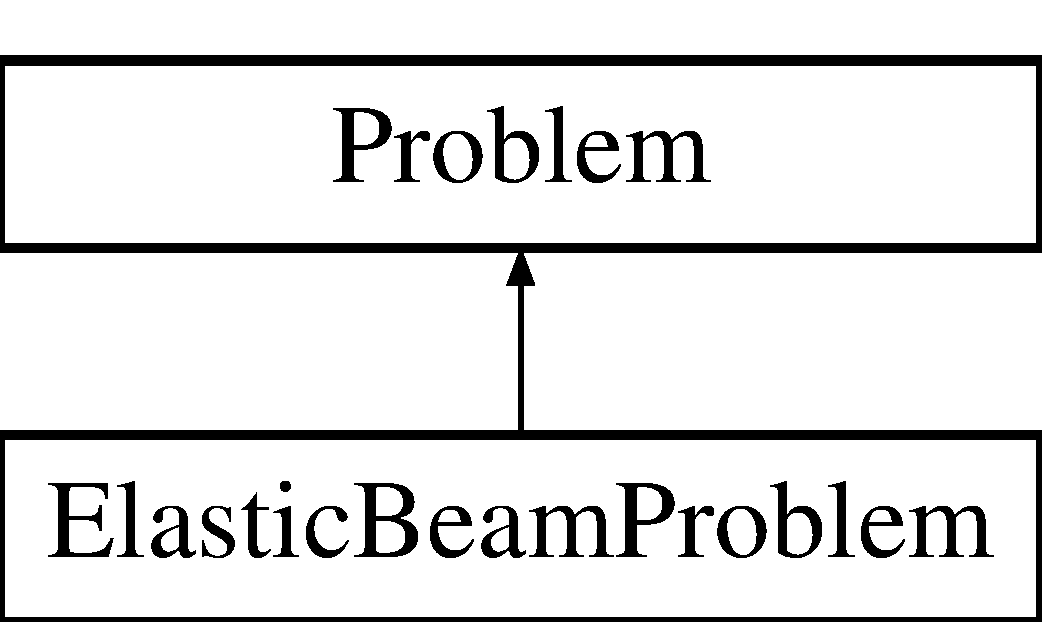
\includegraphics[height=2.000000cm]{classElasticBeamProblem}
\end{center}
\end{figure}
\subsection*{Public Member Functions}
\begin{DoxyCompactItemize}
\item 
\hyperlink{classElasticBeamProblem_a1c62c2a14c9a5528a649700d16dac2ea}{Elastic\+Beam\+Problem} (const unsigned \&n\+\_\+elem, const double \&length)
\begin{DoxyCompactList}\small\item\em Constructor\+: The arguments are the number of elements, the length of domain. \end{DoxyCompactList}\item 
void \hyperlink{classElasticBeamProblem_a2da3cb02ce953da67fb27742e20774a5}{parameter\+\_\+study} ()
\begin{DoxyCompactList}\small\item\em Conduct a parameter study. \end{DoxyCompactList}\item 
One\+D\+Lagrangian\+Mesh$<$ Hermite\+Beam\+Element $>$ $\ast$ \hyperlink{classElasticBeamProblem_ae7d14ba8bec2325a82cbeed0c1b29910}{mesh\+\_\+pt} ()
\begin{DoxyCompactList}\small\item\em Return pointer to the mesh. \end{DoxyCompactList}\item 
void \hyperlink{classElasticBeamProblem_a30dde8d0101a3d3994965d6e560cb585}{actions\+\_\+after\+\_\+newton\+\_\+solve} ()
\begin{DoxyCompactList}\small\item\em No actions need to be performed after a solve. \end{DoxyCompactList}\item 
void \hyperlink{classElasticBeamProblem_a5b534c11d9b1d54123bf587aad5f98f6}{actions\+\_\+before\+\_\+newton\+\_\+solve} ()
\begin{DoxyCompactList}\small\item\em No actions need to be performed before a solve. \end{DoxyCompactList}\end{DoxyCompactItemize}
\subsection*{Private Attributes}
\begin{DoxyCompactItemize}
\item 
Node $\ast$ \hyperlink{classElasticBeamProblem_a9c96cab7e71243e51f7c4040a84cdd5d}{Doc\+\_\+node\+\_\+pt}
\begin{DoxyCompactList}\small\item\em Pointer to the node whose displacement is documented. \end{DoxyCompactList}\item 
double \hyperlink{classElasticBeamProblem_aa68b1c77e0aa1571fe956d62bd8cf096}{Length}
\begin{DoxyCompactList}\small\item\em Length of domain (in terms of the Lagrangian coordinates) \end{DoxyCompactList}\item 
Geom\+Object $\ast$ \hyperlink{classElasticBeamProblem_a134a789cae77ab61a3e32bd93b28e1fa}{Undef\+\_\+beam\+\_\+pt}
\begin{DoxyCompactList}\small\item\em Pointer to geometric object that represents the beam\textquotesingle{}s undeformed shape. \end{DoxyCompactList}\end{DoxyCompactItemize}


\subsection{Detailed Description}
Beam problem object. 

Definition at line 67 of file tensioned\+\_\+string.\+cc.



\subsection{Constructor \& Destructor Documentation}
\mbox{\Hypertarget{classElasticBeamProblem_a1c62c2a14c9a5528a649700d16dac2ea}\label{classElasticBeamProblem_a1c62c2a14c9a5528a649700d16dac2ea}} 
\index{Elastic\+Beam\+Problem@{Elastic\+Beam\+Problem}!Elastic\+Beam\+Problem@{Elastic\+Beam\+Problem}}
\index{Elastic\+Beam\+Problem@{Elastic\+Beam\+Problem}!Elastic\+Beam\+Problem@{Elastic\+Beam\+Problem}}
\subsubsection{\texorpdfstring{Elastic\+Beam\+Problem()}{ElasticBeamProblem()}}
{\footnotesize\ttfamily Elastic\+Beam\+Problem\+::\+Elastic\+Beam\+Problem (\begin{DoxyParamCaption}\item[{const unsigned \&}]{n\+\_\+elem,  }\item[{const double \&}]{length }\end{DoxyParamCaption})}



Constructor\+: The arguments are the number of elements, the length of domain. 

Constructor for elastic beam problem. 

Definition at line 106 of file tensioned\+\_\+string.\+cc.



References Doc\+\_\+node\+\_\+pt, Global\+\_\+\+Physical\+\_\+\+Variables\+::H, Global\+\_\+\+Physical\+\_\+\+Variables\+::load(), mesh\+\_\+pt(), Global\+\_\+\+Physical\+\_\+\+Variables\+::\+Sigma0, and Undef\+\_\+beam\+\_\+pt.



\subsection{Member Function Documentation}
\mbox{\Hypertarget{classElasticBeamProblem_a30dde8d0101a3d3994965d6e560cb585}\label{classElasticBeamProblem_a30dde8d0101a3d3994965d6e560cb585}} 
\index{Elastic\+Beam\+Problem@{Elastic\+Beam\+Problem}!actions\+\_\+after\+\_\+newton\+\_\+solve@{actions\+\_\+after\+\_\+newton\+\_\+solve}}
\index{actions\+\_\+after\+\_\+newton\+\_\+solve@{actions\+\_\+after\+\_\+newton\+\_\+solve}!Elastic\+Beam\+Problem@{Elastic\+Beam\+Problem}}
\subsubsection{\texorpdfstring{actions\+\_\+after\+\_\+newton\+\_\+solve()}{actions\_after\_newton\_solve()}}
{\footnotesize\ttfamily void Elastic\+Beam\+Problem\+::actions\+\_\+after\+\_\+newton\+\_\+solve (\begin{DoxyParamCaption}{ }\end{DoxyParamCaption})\hspace{0.3cm}{\ttfamily [inline]}}



No actions need to be performed after a solve. 



Definition at line 84 of file tensioned\+\_\+string.\+cc.

\mbox{\Hypertarget{classElasticBeamProblem_a5b534c11d9b1d54123bf587aad5f98f6}\label{classElasticBeamProblem_a5b534c11d9b1d54123bf587aad5f98f6}} 
\index{Elastic\+Beam\+Problem@{Elastic\+Beam\+Problem}!actions\+\_\+before\+\_\+newton\+\_\+solve@{actions\+\_\+before\+\_\+newton\+\_\+solve}}
\index{actions\+\_\+before\+\_\+newton\+\_\+solve@{actions\+\_\+before\+\_\+newton\+\_\+solve}!Elastic\+Beam\+Problem@{Elastic\+Beam\+Problem}}
\subsubsection{\texorpdfstring{actions\+\_\+before\+\_\+newton\+\_\+solve()}{actions\_before\_newton\_solve()}}
{\footnotesize\ttfamily void Elastic\+Beam\+Problem\+::actions\+\_\+before\+\_\+newton\+\_\+solve (\begin{DoxyParamCaption}{ }\end{DoxyParamCaption})\hspace{0.3cm}{\ttfamily [inline]}}



No actions need to be performed before a solve. 



Definition at line 87 of file tensioned\+\_\+string.\+cc.

\mbox{\Hypertarget{classElasticBeamProblem_ae7d14ba8bec2325a82cbeed0c1b29910}\label{classElasticBeamProblem_ae7d14ba8bec2325a82cbeed0c1b29910}} 
\index{Elastic\+Beam\+Problem@{Elastic\+Beam\+Problem}!mesh\+\_\+pt@{mesh\+\_\+pt}}
\index{mesh\+\_\+pt@{mesh\+\_\+pt}!Elastic\+Beam\+Problem@{Elastic\+Beam\+Problem}}
\subsubsection{\texorpdfstring{mesh\+\_\+pt()}{mesh\_pt()}}
{\footnotesize\ttfamily One\+D\+Lagrangian\+Mesh$<$Hermite\+Beam\+Element$>$$\ast$ Elastic\+Beam\+Problem\+::mesh\+\_\+pt (\begin{DoxyParamCaption}{ }\end{DoxyParamCaption})\hspace{0.3cm}{\ttfamily [inline]}}



Return pointer to the mesh. 



Definition at line 79 of file tensioned\+\_\+string.\+cc.



Referenced by Elastic\+Beam\+Problem(), and parameter\+\_\+study().

\mbox{\Hypertarget{classElasticBeamProblem_a2da3cb02ce953da67fb27742e20774a5}\label{classElasticBeamProblem_a2da3cb02ce953da67fb27742e20774a5}} 
\index{Elastic\+Beam\+Problem@{Elastic\+Beam\+Problem}!parameter\+\_\+study@{parameter\+\_\+study}}
\index{parameter\+\_\+study@{parameter\+\_\+study}!Elastic\+Beam\+Problem@{Elastic\+Beam\+Problem}}
\subsubsection{\texorpdfstring{parameter\+\_\+study()}{parameter\_study()}}
{\footnotesize\ttfamily void Elastic\+Beam\+Problem\+::parameter\+\_\+study (\begin{DoxyParamCaption}{ }\end{DoxyParamCaption})}



Conduct a parameter study. 

Solver loop to perform parameter study. 

Definition at line 176 of file tensioned\+\_\+string.\+cc.



References Doc\+\_\+node\+\_\+pt, Global\+\_\+\+Physical\+\_\+\+Variables\+::H, Length, mesh\+\_\+pt(), Global\+\_\+\+Physical\+\_\+\+Variables\+::\+P\+\_\+ext, and Global\+\_\+\+Physical\+\_\+\+Variables\+::\+Sigma0.



Referenced by main().



\subsection{Member Data Documentation}
\mbox{\Hypertarget{classElasticBeamProblem_a9c96cab7e71243e51f7c4040a84cdd5d}\label{classElasticBeamProblem_a9c96cab7e71243e51f7c4040a84cdd5d}} 
\index{Elastic\+Beam\+Problem@{Elastic\+Beam\+Problem}!Doc\+\_\+node\+\_\+pt@{Doc\+\_\+node\+\_\+pt}}
\index{Doc\+\_\+node\+\_\+pt@{Doc\+\_\+node\+\_\+pt}!Elastic\+Beam\+Problem@{Elastic\+Beam\+Problem}}
\subsubsection{\texorpdfstring{Doc\+\_\+node\+\_\+pt}{Doc\_node\_pt}}
{\footnotesize\ttfamily Node$\ast$ Elastic\+Beam\+Problem\+::\+Doc\+\_\+node\+\_\+pt\hspace{0.3cm}{\ttfamily [private]}}



Pointer to the node whose displacement is documented. 



Definition at line 92 of file tensioned\+\_\+string.\+cc.



Referenced by Elastic\+Beam\+Problem(), and parameter\+\_\+study().

\mbox{\Hypertarget{classElasticBeamProblem_aa68b1c77e0aa1571fe956d62bd8cf096}\label{classElasticBeamProblem_aa68b1c77e0aa1571fe956d62bd8cf096}} 
\index{Elastic\+Beam\+Problem@{Elastic\+Beam\+Problem}!Length@{Length}}
\index{Length@{Length}!Elastic\+Beam\+Problem@{Elastic\+Beam\+Problem}}
\subsubsection{\texorpdfstring{Length}{Length}}
{\footnotesize\ttfamily double Elastic\+Beam\+Problem\+::\+Length\hspace{0.3cm}{\ttfamily [private]}}



Length of domain (in terms of the Lagrangian coordinates) 



Definition at line 95 of file tensioned\+\_\+string.\+cc.



Referenced by parameter\+\_\+study().

\mbox{\Hypertarget{classElasticBeamProblem_a134a789cae77ab61a3e32bd93b28e1fa}\label{classElasticBeamProblem_a134a789cae77ab61a3e32bd93b28e1fa}} 
\index{Elastic\+Beam\+Problem@{Elastic\+Beam\+Problem}!Undef\+\_\+beam\+\_\+pt@{Undef\+\_\+beam\+\_\+pt}}
\index{Undef\+\_\+beam\+\_\+pt@{Undef\+\_\+beam\+\_\+pt}!Elastic\+Beam\+Problem@{Elastic\+Beam\+Problem}}
\subsubsection{\texorpdfstring{Undef\+\_\+beam\+\_\+pt}{Undef\_beam\_pt}}
{\footnotesize\ttfamily Geom\+Object$\ast$ Elastic\+Beam\+Problem\+::\+Undef\+\_\+beam\+\_\+pt\hspace{0.3cm}{\ttfamily [private]}}



Pointer to geometric object that represents the beam\textquotesingle{}s undeformed shape. 



Definition at line 98 of file tensioned\+\_\+string.\+cc.



Referenced by Elastic\+Beam\+Problem().



The documentation for this class was generated from the following file\+:\begin{DoxyCompactItemize}
\item 
\hyperlink{tensioned__string_8cc}{tensioned\+\_\+string.\+cc}\end{DoxyCompactItemize}

\chapter{File Documentation}
\hypertarget{tensioned__string_8cc}{}\section{tensioned\+\_\+string.\+cc File Reference}
\label{tensioned__string_8cc}\index{tensioned\+\_\+string.\+cc@{tensioned\+\_\+string.\+cc}}
\subsection*{Classes}
\begin{DoxyCompactItemize}
\item 
class \hyperlink{classElasticBeamProblem}{Elastic\+Beam\+Problem}
\begin{DoxyCompactList}\small\item\em Beam problem object. \end{DoxyCompactList}\end{DoxyCompactItemize}
\subsection*{Namespaces}
\begin{DoxyCompactItemize}
\item 
 \hyperlink{namespaceGlobal__Physical__Variables}{Global\+\_\+\+Physical\+\_\+\+Variables}
\begin{DoxyCompactList}\small\item\em Namespace for physical parameters. \end{DoxyCompactList}\end{DoxyCompactItemize}
\subsection*{Functions}
\begin{DoxyCompactItemize}
\item 
void \hyperlink{namespaceGlobal__Physical__Variables_a321267e1efb30b5d586302509354fb07}{Global\+\_\+\+Physical\+\_\+\+Variables\+::load} (const Vector$<$ double $>$ \&xi, const Vector$<$ double $>$ \&x, const Vector$<$ double $>$ \&N, Vector$<$ double $>$ \&load)
\begin{DoxyCompactList}\small\item\em Load function\+: Apply a constant external pressure to the beam. \end{DoxyCompactList}\item 
int \hyperlink{tensioned__string_8cc_ae66f6b31b5ad750f1fe042a706a4e3d4}{main} ()
\begin{DoxyCompactList}\small\item\em Driver for beam (string under tension) test problem. \end{DoxyCompactList}\end{DoxyCompactItemize}
\subsection*{Variables}
\begin{DoxyCompactItemize}
\item 
double \hyperlink{namespaceGlobal__Physical__Variables_af6e07423e22c0991084d9a2f43727805}{Global\+\_\+\+Physical\+\_\+\+Variables\+::H}
\begin{DoxyCompactList}\small\item\em Non-\/dimensional thickness. \end{DoxyCompactList}\item 
double \hyperlink{namespaceGlobal__Physical__Variables_a417dc688a70c4f06ef0faed047068ba2}{Global\+\_\+\+Physical\+\_\+\+Variables\+::\+Sigma0}
\begin{DoxyCompactList}\small\item\em 2nd Piola Kirchhoff pre-\/stress \end{DoxyCompactList}\item 
double \hyperlink{namespaceGlobal__Physical__Variables_a0406c0cbd463d1df2458fe5de98a00eb}{Global\+\_\+\+Physical\+\_\+\+Variables\+::\+P\+\_\+ext}
\begin{DoxyCompactList}\small\item\em Pressure load. \end{DoxyCompactList}\end{DoxyCompactItemize}


\subsection{Function Documentation}
\mbox{\Hypertarget{tensioned__string_8cc_ae66f6b31b5ad750f1fe042a706a4e3d4}\label{tensioned__string_8cc_ae66f6b31b5ad750f1fe042a706a4e3d4}} 
\index{tensioned\+\_\+string.\+cc@{tensioned\+\_\+string.\+cc}!main@{main}}
\index{main@{main}!tensioned\+\_\+string.\+cc@{tensioned\+\_\+string.\+cc}}
\subsubsection{\texorpdfstring{main()}{main()}}
{\footnotesize\ttfamily int main (\begin{DoxyParamCaption}{ }\end{DoxyParamCaption})}



Driver for beam (string under tension) test problem. 



Definition at line 261 of file tensioned\+\_\+string.\+cc.



References Global\+\_\+\+Physical\+\_\+\+Variables\+::H, Elastic\+Beam\+Problem\+::parameter\+\_\+study(), and Global\+\_\+\+Physical\+\_\+\+Variables\+::\+Sigma0.


\hypertarget{tensioned__string_8txt__doxygenified_8h}{}\section{tensioned\+\_\+string.\+txt\+\_\+doxygenified.\+h File Reference}
\label{tensioned__string_8txt__doxygenified_8h}\index{tensioned\+\_\+string.\+txt\+\_\+doxygenified.\+h@{tensioned\+\_\+string.\+txt\+\_\+doxygenified.\+h}}

%--- End generated contents ---

% Index
\backmatter
\newpage
\phantomsection
\clearemptydoublepage
\addcontentsline{toc}{chapter}{Index}
\printindex

\end{document}
